\documentclass[../main.tex]{subfiles}

\begin{document}
\section{Previous Drag Analysis}

Before knowing that the airship envelope needed to be parametrizable, drag values were initially computed using SolidWorks, by its built in Flow Simulation add-on. Simulations were conducted from 2m/s to 20m/s, at intervals of 2m/s. Skin Friction Drag and Regular Drag were computed and summed to obtain total drag for each speed. A table with the results from the simulations can be seen in Table \ref{tbl:DracTable}.

\begin{table}[H]
	\centering
	\caption{Raw Data From SolidWorks Flow Simulation}
	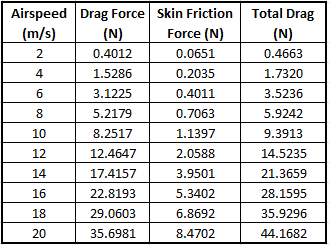
\includegraphics[width=.5\linewidth]{img/drag/dragTable.PNG}
	\label{tbl:DracTable}
\end{table}

\begin{figure}[H]
	\centering
	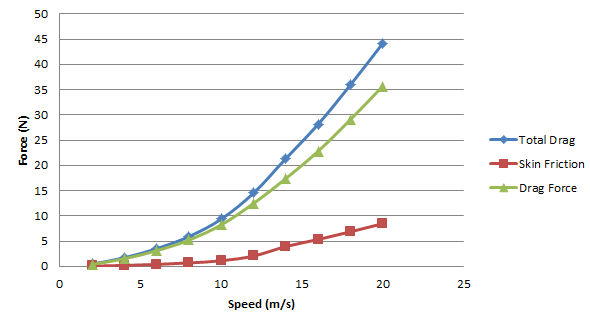
\includegraphics[width=\linewidth]{img/drag/dragForces.PNG}
	\caption{Drag Force Curves Computed From SolidWorks Flow Simulation}
	\label{fig:dragForces}
\end{figure}

The values of simulated drag were then sent into MATLAB and a curve fitting analysis was completed. A graph of the raw data versus the fitted curve is shown in Figure \ref{fig:dragForces}.

\begin{figure}[H]
	\centering
	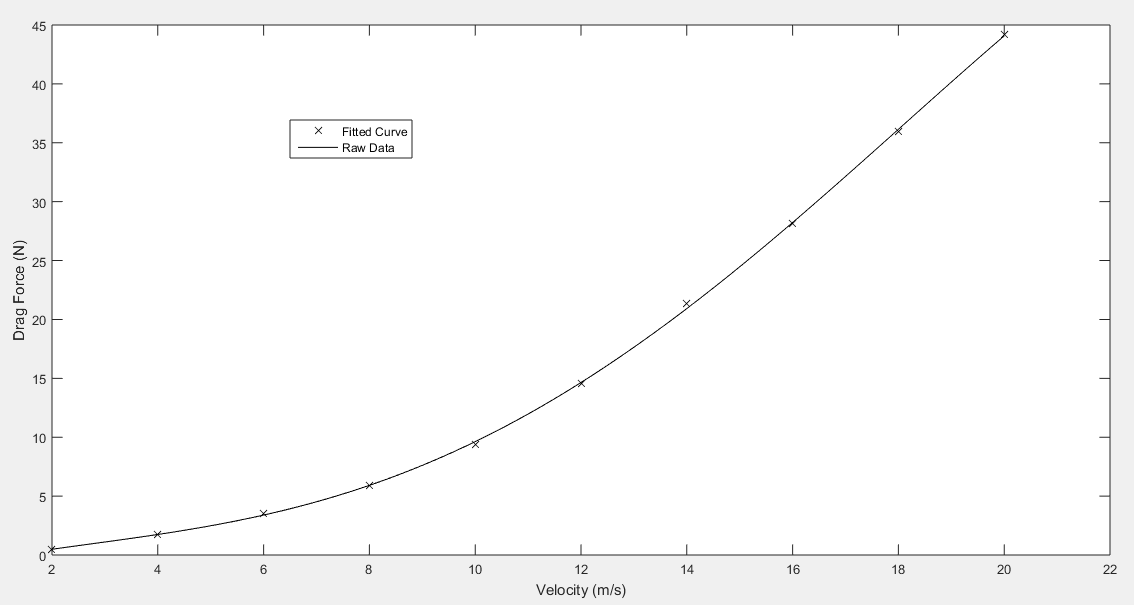
\includegraphics[width=\linewidth]{img/drag/curveFit.PNG}
	\caption{Drag Force Curves Computed From SolidWorks Flow Simulation}
	\label{fig:curveFit}
\end{figure}

The equation from the curve (generated from MATLAB) was found to be:

\begin{equation} \label{dragEqn}
	D(v) = -0.0003545v^4 + 0.014182v^3 -0.05385v^2 + 0.45054v -0.087259
\end{equation}

Where $ D $ is the drag force and $ v $ is the airship speed, in $m/s$. Equation \ref{dragEqn} is what is used throughout the report to obtain drag forces.\\

Raw MATLAB code:

\lstinputlisting[language=Octave]{MATLAB/drag/curveFit.m}

\section{New Drag Analysis}

Once it was understood that the airship itself needed to be parametrizable, a new method of computed drag needed to be determined, as the simulations only accounted for the old airship dimensions. For this, an analysis from a report called \textit{Technical Manual of Airship Aerodynamics} \cite{airshipAerodynamics} was used. The following forumla was used to compute drag:

\begin{equation}
		D = C_D\rho (vol)^{2/3}v^{1.86}
\end{equation}

Where $D$ is the drag in $lbf$ (converted to N), $ \rho $ is the density of air $[slugs/ft^3]$, $vol$ is the volume of the airship envelope $[ft^3]$, $v$ is the velocity of the airship $[ft/s]$, and $C_D$ is the Prandtl Shape Coefficient. For this airship, $C_D$ is estimated using Table \ref{tbl:airshipTable} below.

\begin{table}[H]
	\centering
	\caption{Airship Model Characteristics and Data \cite{airshipAerodynamics}}
	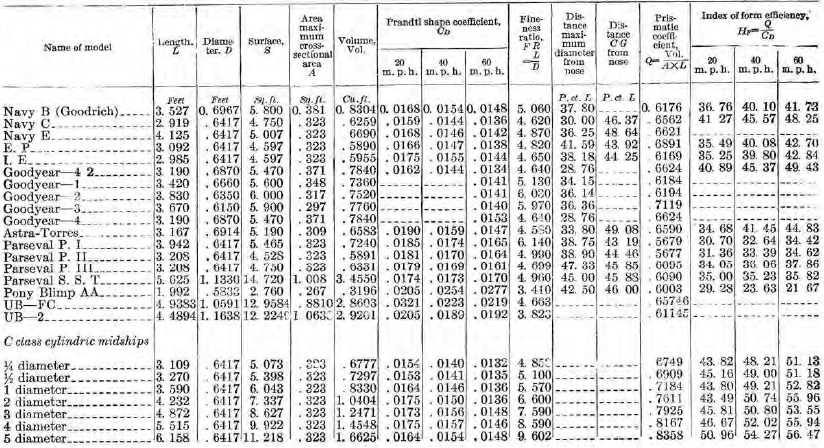
\includegraphics[width=\linewidth]{img/drag/airships.PNG}
	\label{tbl:airshipTable}
\end{table}

Various airship dimensions can be seen below here. The aircraft dimensions shown below were for testing done in a wind tunnel to determine drag effects on real airships, so they are scaled down models. The goal is to select a model that has comparable dimensions to the airship we are using. As a starting point, the fineness ratio $f$ is computed for out airship. As an estimate, $f=L/D \approx 3.6/1.2 = 3$. In reference to Table \ref{tbl:airshipTable}, the closest match would be the Pony Blimp AA, with a fineness ratio of 3.4.\\

It can be deduced from the table that the Prandtl Shape coefficient encompasses both skin and form drag. When the fineness ratio is higher, skin friction drag will have a larger effect than form drag, so when the airspeed is increased (from 20mph to 60mph), $C_D$ will decrease. The opposite is true with small fineness ratios, where the form drag plays a larger role, therefore the $C_D$ increases as airspeed is increased. To be conservative, the highest $C_D$ from the Pony Blimp AA, therefore $C_D = 0.0227$. An example calculation is shown below, for a windspeed of $20m/s$:
\begin{equation} \label{exDrag}
D = C_D\rho (vol)^{2/3}v^{1.86}=0.0227*(0.00237 slugs/ft^3)*(122.644 ft^3)^{2/3}(65.616 ft/s) ^{1.86} = 3.183 lbf = 14.1586N 
\end{equation}

The formula will is converted into metric units for simplicity, using a multiplication factor.
\begin{equation}
D = 0.847103*(C_D)*(\rho[kg/m^3])*(vol [m^3])^{2/3}*(v [m/s])^{1.86}
\end{equation}

Based on Table \ref{tbl:contributionsTable}, the envelope contributes 45\% to the drag. Therefore the total drag will be estimated as $D_{total}=D/0.45$. Based on this, the total drag in found in Equation \ref{exDrag} is now $31.463N$

\begin{table}[H]
	\centering
	\caption{Drag Contribution for Various Airship Components \cite{airshipAerodynamics}}
	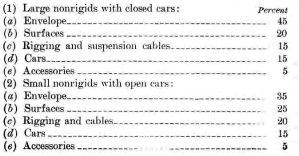
\includegraphics[width=.5\linewidth]{img/drag/contributions.PNG}
	\label{tbl:contributionsTable}
\end{table}

The value of $C_D$ will change based on the fineness ratio. In the GUI of the MATLAB program, the user will select a fineness ratio from a drop-down menu, of 3.5, 4, and 4.5, followed by a total length of the blimp. To calculate the drag for these situations, the volume of the blimp will be computed, and the $C_D$ will change based on the fineness ratio, as follows:
\begin{table}[H]
	\caption{Fineness Ratios and Corresponding $C_D$}
	\label{tbl:finenessCoefficient}
\begin{center}
	\begin{tabular}{|c|c|}
	\hline 
	\textbf{Fineness Ratio} & \textbf{$C_D$} \\ 
	\hline 
	3.5 & 0.0254 \\ 
	\hline 
	4 & 0.0189 \\ 
	\hline 
	4.5 & 0.0159 \\ 
	\hline 
\end{tabular} 
\end{center}
\end{table}

\end{document}